\documentclass[
	% -- opções da classe memoir --
	article,			% indica que é um artigo acadêmico
	11pt,				% tamanho da fonte
	oneside,			% para impressão apenas no recto. Oposto a twoside
	a4paper,			% tamanho do papel.
	openany,
	% -- opções da classe abntex2 --
	%chapter=TITLE,		% títulos de capítulos convertidos em letras maiúsculas
	%section=TITLE,		% títulos de seções convertidos em letras maiúsculas
	%subsection=TITLE,	% títulos de subseções convertidos em letras maiúsculas
	%subsubsection=TITLE % títulos de sub subseções convertidos em letras maiúsculas
	% -- opções do pacote babel --
	english,			% idioma adicional para hifenização
	brazil,				% o último idioma é o principal do documento
	sumario=tradicional
	]{abntex2}
% ---
% PACOTES
% ---
\usepackage{lmodern}			% Usa a fonte Latin Modern
\usepackage[T1]{fontenc}		% Seleção de códigos de fonte.
\usepackage[utf8]{inputenc}		% Codificação do documento (conversão automática dos acentos)
\usepackage{indentfirst}		% Indenta o primeiro parágrafo de cada seção.
\usepackage{nomencl} 			% Lista de símbolos
\usepackage{color}				% Controle das cores
\usepackage{graphicx}			% Inclusão de gráficos
\usepackage{microtype} 			% para melhorias de justificação
\usepackage{lipsum}				% para geração de dummy text
\usepackage{float}				% para geração de dummy text
\graphicspath{ {./imgs/} }
\usepackage[
	style=abnt,
	backref=true,
]{biblatex}
\addbibresource{~/.bibli.bib}
\usepackage{hyperref}

% --- Informações de dados para CAPA e FOLHA DE ROSTO ---
\titulo{Reconhecimente de números usando Redes Neurais Artificiais}
\tituloestrangeiro{}

\autor{ Mario Moura \and Pedro Honório}

\local{Brasil}
\data{\today}
% ---
% ---
% Configurações de aparência do PDF final
% alterando o aspecto da cor azul
\definecolor{blue}{RGB}{41,5,195}
% informações do PDF
\makeatletter
\hypersetup{
	%pagebackref=true,
	pdftitle={\@title},
	pdfauthor={\@author},
	pdfsubject={Modelo de artigo científico com abnTeX2},
	pdfcreator={LaTeX with abnTeX2},
	pdfkeywords={abnt}{latex}{abntex}{abntex2}{atigo científico},
	colorlinks=true,	% false: boxed links; true: colored links
	linkcolor=blue,          	% color of internal links
	citecolor=blue,        		% color of links to bibliography
	filecolor=magenta,      		% color of file links
	urlcolor=blue,
	bookmarksdepth=4
}
\makeatother
% ---

% ---
% compila o índice
% ---
\makeindex
% ---

% ---
% Altera as margens padrões
% ---
\setlrmarginsandblock{3cm}{3cm}{*}
\setulmarginsandblock{3cm}{3cm}{*}
\checkandfixthelayout
% ---

% ---
% Espaçamentos entre linhas e parágrafos
% ---

% O tamanho do parágrafo é dado por:
\setlength{\parindent}{1.3cm}

% Controle do espaçamento entre um parágrafo e outro:
\setlength{\parskip}{0.2cm}  % tente também \onelineskip

% Espaçamento simples
\SingleSpacing

% ----
% Início do documento
% ----
\begin{document}

% Seleciona o idioma do documento (conforme pacotes do babel)
%\selectlanguage{english}
\selectlanguage{brazil}
% Retira espaço extra obsoleto entre as frases.
\frenchspacing
% ----------------------------------------------------------
% ELEMENTOS PRÉ-TEXTUAIS
% ----------------------------------------------------------
% página de titulo principal (obrigatório)
\maketitle

% resumo em português
\begin{resumoumacoluna}
	Um dos tópicos clássicos que exploram o poder das redes neurais
	sem se perder na complexidade é a identificação de símbolos e
	hieroglifos. Tarefa que a olhos destreinados pode parecer
	extremamente trivial, entretanto quando examinada mais de
	perto se torna algo inimaginável para se traduzir de uma
	maneira imperativa. A técnica de representar problemas
	com pseudo neurónios e alterar o processamento deles através
	do \emph{backpropagation} veio para auxiliar em tarefas muito
	abstratas. Utilizando essas técnicas é possível identificar
	números simples de zero à nove.

	\vspace{\onelineskip}
	\noindent
	\textbf{Palavras-chave}: Redes Neurais. Inteligência Artificial. Python.
\end{resumoumacoluna}


% ----------------------------------------------------------
% ELEMENTOS TEXTUAIS
% ----------------------------------------------------------
\textual

% ----------------------------------------------------------
% Introdução
% ----------------------------------------------------------
\section{Problema}
O problema da identificação de algarismos de zero(0) à nove(9)
tem como objetivo a classificação de imagens, com resolução
\(28\times28\)\emph{pixels}, em uma das 10 categorias. Cada
uma representando um número de um dígito. São necessários então
imagens de dígitos escritos as mão e suas respectivas respostas.
O \emph{DeepAi}\footnote{\url{https://deepai.org}}
disponibiliza um conjunto de dados batizado de ``\emph{MNIST}'',
contendo 60000 exemplos para treinamento e 10000 exemplos para
teste.

\subsection{Arquitetura RNA}
Como as imagens possuem \(28\times28\) de resolução, cada uma
representa 784 \emph{pixels} obtendo-se 784 neurônios de entrada
e como são dez possíveis classificações foi escolhido 10 neurônios
como saída. O algoritmo de \emph{stochastic gradient descent} foi
escolhido utilizando uma função sigmoidal como processamento dos
neurônios.

Todos os neurônios aceitam pontos flutuantes de 0.00 à 1.00
e retornam também números de 0.00 à 1.00.

\subsection{Tratamento de Codificação de dados}
O \emph{set} de dados do MNIST provém vetores representando
cada, os \emph{pixels} das imagens, variando entre 0 e 255 numa escala
de quão cinza é aquele pixel, sendo 0 para totalmente preto e 255
para branco. Esses são os arquivos intitulados ``\emph{images}''.
Os outros arquivos, intitulados de ``\emph{labels}'' são as repostas
das suas respectivas imagens, também num formato vetorial.

O Vetor de imagens é transformado num vetor de x entradas sendo x
o número de imagens no arquivo e cada entrada sendo um outro vetor
contendo os \emph{pixels} de uma imagem em sequência, então as
respostas serão transformadas em vetores com dez posições zeradas
onde apenas a posição cujo o índice é a resposta recebe o valor um.
Finalmente a matriz de \emph{pixels} é associada ao vetor de
respostas(lembrando que cada entrada no vetor de respostas é um
vetor de 10 posições) no formato de lista.

\begin{itemize}
	\item Matriz de treino (\(60000\times784\)):
		[[0,0,...,254,...,0],[0,0,...,125,194,255,...,0,0],...]
	\item Matriz de respostas (\(60000\times10\)):
		[[0,0,0,0,0,0,0,1,0,0,],...,[0,0,1,0,0,0,0,0,0,0,]]
	\item Matriz de teste (\(10000\times784\)):
		[[0,0,...,254,...,0],[0,0,...,125,194,255,...,0,0],...]
	\item Vetor de respostas (\(10000\)):
		[2,5,4,7,3,0,9,1,6,3,...,4,1,3,2,0,7,8,3,7,4]
\end{itemize}

Todas as matrizes podem ser encontradas no site do
\emph{DeepAi}\footnote{\url{https://deepai.org/dataset/mnist}}
na forma vetorial de e num arquivo binário.

\section{Implementação}

\begin{table}[h]
	\centering
	\begin{tabular}{||c|c|c|c|c||}
		\hline
			Rede & Camada Intermediária & Taxa de aprendizagem & Épocas & Taxa de Acerto \\
		\hline\hline
			A & 10 & 0.1 & 5 & 80.38\% \\
		\hline
			B & 15 & 0.2 & 5 & 87.37\% \\
		\hline
			C & 15 & 0.2 & 10 & 89.37\% \\
		\hline
			D & 15, 15 & 0,3 & 10 & 90.64\% \\
		\hline
			E & 30, 30 & 0,5 & 10 & 93.28\% \\
		\hline
			F & 50, 50 & 0,7 & 10 & 94.43\% \\
		\hline
	\end{tabular}
	%\caption{Tabela de cronograma}
	%\label{cronograma}
\end{table}

\begin{figure}[H]
	\centering
	\caption{Evolução das redes por época}
	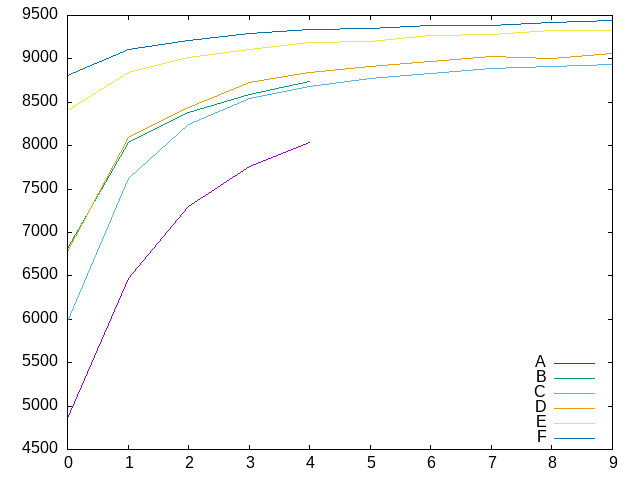
\includegraphics[scale = 0.75]{Redes.png}
	\label{Redes}
	\centering
\end{figure}

\section{Análise dos Resultados}
Todos os resultados foram relativamente aceitáveis, entretanto devido
a grande quantidade de dados não foi necessário muitas épocas.
Foi escolhido nesse caso utilizar-se de múltiplas camadas ao
invés de uma única camada gigante justamente pela grande camada de
neurônios iniciais. Uma grande dificuldade do modelo é superar
taxas de aceto superiores à 90\%, à solução foi justamente aumentar
o numero de camadas intermediárias juntamente com a taxa de aprendizado
levemente.

Interessante notar as curvas das redes no gráfico \ref{Redes}, que
obedecem um padrão de declínio. Outro detalhe interessante à se notar
é a simplicidade do algorítimo que se faz eficaz justamente pela grande
disponibilidade de dados para ser treinado.


\begin{apendicesenv}

\chapter{Scripts}

\end{apendicesenv}


\end{document}
